%コンパイル方法: opt+cmd+b → opt+cmd+v
\RequirePackage{plautopatch}

\documentclass[a4paper, 9pt]{ltjsarticle}


% マージン設定
\usepackage[top=20mm, bottom=20mm, left=20mm, right=20mm]{geometry}

% LuaLaTeX用日本語対応パッケージ
\usepackage{luatexja}
\usepackage{luatexja-fontspec}

% 必要なパッケージ
\usepackage{fontspec}
\usepackage{titlesec}
\usepackage{graphicx}
\usepackage{amsmath}
\usepackage{amssymb}
\usepackage[hidelinks]{hyperref}
\usepackage[english, japanese]{babel}
\usepackage{multicol} % 二段組用パッケージ
\usepackage{indentfirst}
\usepackage{tikz} % カスタム点線用
\usepackage{authblk} % 著者・所属パッケージ
\usepackage{here}
\usepackage{caption}
\usepackage{bookmark}
\usepackage{array}
\usepackage{diagbox} % 斜線を入れるためのパッケージ


% \setmainfont[Ligatures=TeX]{Times New Roman}
% \setmainjfont[BoldFont=MS Gothic]{MS Mincho}

\renewcommand{\baselinestretch}{0.95}
\renewcommand{\labelenumi}{(\arabic{enumi})}

% セクション見出しのカスタマイズ
\titleformat{\section}
  {\fontsize{10pt}{10pt}}
  {\thesection.}
  {1em}{}

\titleformat{\subsection}
  {\fontsize{10pt}{10pt}}
  {\thesubsection}
  {1em}{}

\titleformat{\subsubsection}
  {\fontsize{10pt}{10pt}}
  {\thesubsubsection}
  {1em}{}

  \setlength{\parindent}{1em}
% \setlength{\belowcaptionskip}{1em} % キャプション下の余白を -10pt に設定


%section前に余白を作る
\titlespacing*{\section}{0em}{1em}{0em}
\titlespacing*{\subsection}{0em}{1em}{0em}
\titlespacing*{\subsubsection}{0em}{1em}{0em}

\pagestyle{empty}


\begin{document}

\setlength{\columnsep}{7.5mm}

\twocolumn[
    \begin{center}
        {\vspace{-1em}}

        {\fontsize{15pt}{15pt}\selectfont{災害時を想定したアドホックネットワーク構築手法の検討}}

        {\vspace{1.5em}}

        {\fontsize{13pt}{13pt}\selectfont{A study of ad hoc network construction methods for disaster scenarios}}
    \end{center}



    \begin{flushright}
      {\fontsize{11pt}{11pt}\selectfont{T5-17 末廣隼人\\}}
      {\fontsize{11pt}{11pt}\selectfont{指導教員 髙﨑和之}}
    \end{flushright}

    \vspace{1em}

    \thispagestyle{empty}
]

\section{はじめに}

% 自然災害、特に地震発生時に基地局の倒壊やネットワーク障害が生じたときに、
% その間に助けを求める人達の不安を少しでも拭うために一時的なネットワーク、
% アドホックネットワークの構築を行い少しでも多くの情報を共有できることを目的として研究を行った。\\
% 具体的には、被災エリアの中心に主となるノードを設置、その周りに携帯端末が保有するBluetoothなどでアドホックネットワークの構築おこうなう。
% このとき、全ての端末をアドホックに使用してしまうと、ルーティングが煩雑distribution化してしまうしまうため、
% アルゴリズムでメインとして使用する端末と接続が切れてしまった時の補助端末に分ける。その方法を第3章で述べる。

% 日本では多くの自然災害が発生しており、自然災害の中で一番恐れらている災害が地震であった。
% 昨年の石川県能登半島で発生した大地震では多くの死傷者がでてしまい、甚大な被害を被った。
% この災害では特に高齢者の人口が多く占めており、迅速な避難が難しかったり、

% \section{研究背景}

\section{理論}
\subsection{アドホックネットワーク}
アドホックネットワークとは、中央の管理者やルータ、アクセスポイント等の既存のインフラストラクチャを介さずに、端末(以降ノードという)同士が直接通信を行う一時的なネットワークのことである。
遠くのノードと通信を行うとき、隣接する他ノードを中継機として利用し、バケツリレーのようにデータを送信するマルチホップ通信技術を用いる。%
\\ \indent 本研究では、低コスト、低消費電力でスマートフォンに内蔵されているBluetoothを用いたアドホックネットワークを想定し、
より消費電力が少ないBluetooth Low Energy(BLE)の接続目安距離である30mを最大通信距離としてシミュレーションを行った。

\subsection{ルーティング制御方法}
各ノードが通信を行う際のルーティング方式には大きく分けてリアクティブ型、プロアクティブ型、ハイブリッド型の3種類がある。
各方式の特徴を次に示す。本研究では、ハイブリッド型を参考に経路生成手法の検討を行なった。
\begin{enumerate}
  \item \label{reactive} リアクティブ型 \par  
  \indent 通信要求が発生した時に近くのノードとその場でデータのやり取りを行い経路を作成する。
  通信開始までに遅延が生じるが経路情報維持のための通信が不要なため通信頻度の低い環境では消費電力が少なく長時間使用できる。
  代表的なプロトコルとしてAODVやDSRなどがある。

  \item \label{proactive} プロアクティブ型 \par
  \indent 近くのノード間で自身の情報をやりとし経路をあらかじめ作成する。あらかじめ経路が作成されるため、通信開始までの遅延が短い。  
  しかし、定期的にデータのやり取りを行うため消費電力が多い。代表的なプロトコルとしてOLSRやTBRPFなどがある。

  \item ハイブリッド型 \par
  \indent (\ref{reactive})、(\ref{proactive}) の二つを組み合わせたルーティング方式である。代表的なプロトコルとしてはZRPなどがある。
\end{enumerate}

\section{提案手法}
\subsection{想定環境}
経路生成のシミュレーションにあたりノードの密度は日本の人口密度に持ち運びが便利なスマートフォンの所有率88.6\%\cite{スマホ保有率}を乗じた数とした。%
人口密度が高い地域として埼玉県、低い地域として福島県、また、昨年被災した石川県羽咋市の3つの地域に対してシミュレーションを行った。
また、人口密度が低い地域ではノード同士の間隔が大きくなってしまうため、電柱にBLE機能を有した低コストの機器(以降電柱ノードという)を設置した2つの場合についてのシミュレーションを行った。\par
ノードは1km四方の範囲内に配置し、その中で中心に近いノードをインターネットにつながるゲートウェイ(以降スタートノードという)として、そこから一番遠いものをターゲットノードとして経路を探索した。\par
電柱の設置間隔は約30m\textasciitilde 50m \cite{電柱設置間隔}であるが、人口密度により増減がバラバラになってしまう。
% そのため、今回はそれぞれの地域の人口密度に電柱一本がカバーする人数[人/本]で割った数を電柱の数とした。
% 以下にそれぞれの地域に対応した数値を載せる。

\begin{table}[h]
  \centering
  \caption{2024年10月1日現在の自治体構成}
  \begin{tabular}{|l|c|c|c|}
      \hline
      \tikz[baseline=0pt]{% 斜線
    \useasboundingbox(0,0);
    \draw(-0.2,0.316)--(3.15,-0.136);} & \textbf{埼玉県} & \textbf{福島県} & \textbf{石川県羽咋市} \\
      \hline
      人口密度 [人/$\mathrm{km}^2$] \cite{人口密度} & 1930 & 126 & 232 \\
      % 電柱カバー人数 & 5 & 0.8 & 1 \\
      \hline
      ノードの数 [個] & 1710 & 112 & 206 \\
      \hline
      電柱ノードの数 [個] & 386 & 158 & 232 \\
      \hline
      ノードの合計 [個] & 2096 & 270 & 438 \\
      \hline
  \end{tabular}
\end{table}

\subsection{提案手法-1}
% 理由
人口密度が高い地域で全てのノードが接続してしまうと経路の複雑化や経路長の冗長化により、通信速度や通信品質の低下が発生してしまう。
これらを解決するために、周辺にいるノードの密度を用いて接続ノード数を制限し経路の単純化を行った。ノードに以下のような条件を設けた。\par
% 概要
経路探索法の大まかな流れとしてはじめに、接続要求を行っているノード(以降上流ノードという)の周辺にいるノード(以降下流ノードという)を集計し、
その時の密度に応じて接続数を変化させるようにした。\par
接続までのやり取りは、上流ノードが下流ノードに対してhelloメッセージを送信し、それを受信した下流ノードはhelloメッセージに加え他ノードとの接続状況の内容を上流ノードに返す。
次に、受信した上流ノードは返信数で下流ノードの数を集計し、高密度であれば一つだけランダムに選択し、低密度であれば複数をランダムに選択して接続を行う。
このようにランダムに接続を行っているため、ループが発生しやすくなっている。そこで、先ほど述べた下流ノードのパケット内容で”他ノードとの接続状況”という項目を
利用する。これは上流ノードがノードを選択する前にその下流ノードを除外し、未接続の下流ノードの中から選択を行うと、ループが発生を抑えることができる。\par
% この提案手法では最適な高密度と低密度の具体的な数値を見つけ、シンプルな経路を発見するのが目的である。
% また、情報を取得する条件として、中心にいる上流ノードがターゲットノードと接続した時として、その時の繋がっているノード全ての密度とターゲットノードまでの最短ホップ数
% で比較を行う。

\subsection{提案手法-1のシミュレーション結果}
この提案手法では人口密度が低い地域ではノード間隔が広くなり経路探索ができないため、人口密度が高い埼玉県でシミュレーションを行った。
接続条件は、他ノードと接続済みのノードを除いた時の周辺ノードの密度が3, 4, 5, 6, 7, 8以上のそれぞれ6つについて行った。
上記の条件が正のときランダムに1つ接続し、負のとき周辺ノード数が2以上ならランダムに2つ接続し、1ならそのノードと接続を行った。\par
シミュレーション結果を図\ref{fig:1}にシミュレーションの様子を図\ref{fig:2}に示した。各条件を10回行いその平均値をプロットした。
図\ref{fig:1}より、ノード密度が6以上の時、接続可能ノードの割合が75.91\%で一番高くなった。
図\ref{fig:2}の左側のグラフは、中心に位置する赤点がスタートノード、少し離れている赤点がターゲットノード、青点が接続可能ノード、オレンジ点が接続不可能ノード、薄青が接続距離である。
また、赤線はスタートノードとターゲットノードの経路である。次に右側のグラフは、各接続可能ノードのノード密度を集計したグラフである。\par

\begin{figure}[ht] % [h]は「ここに表示」の意味
  \centering
  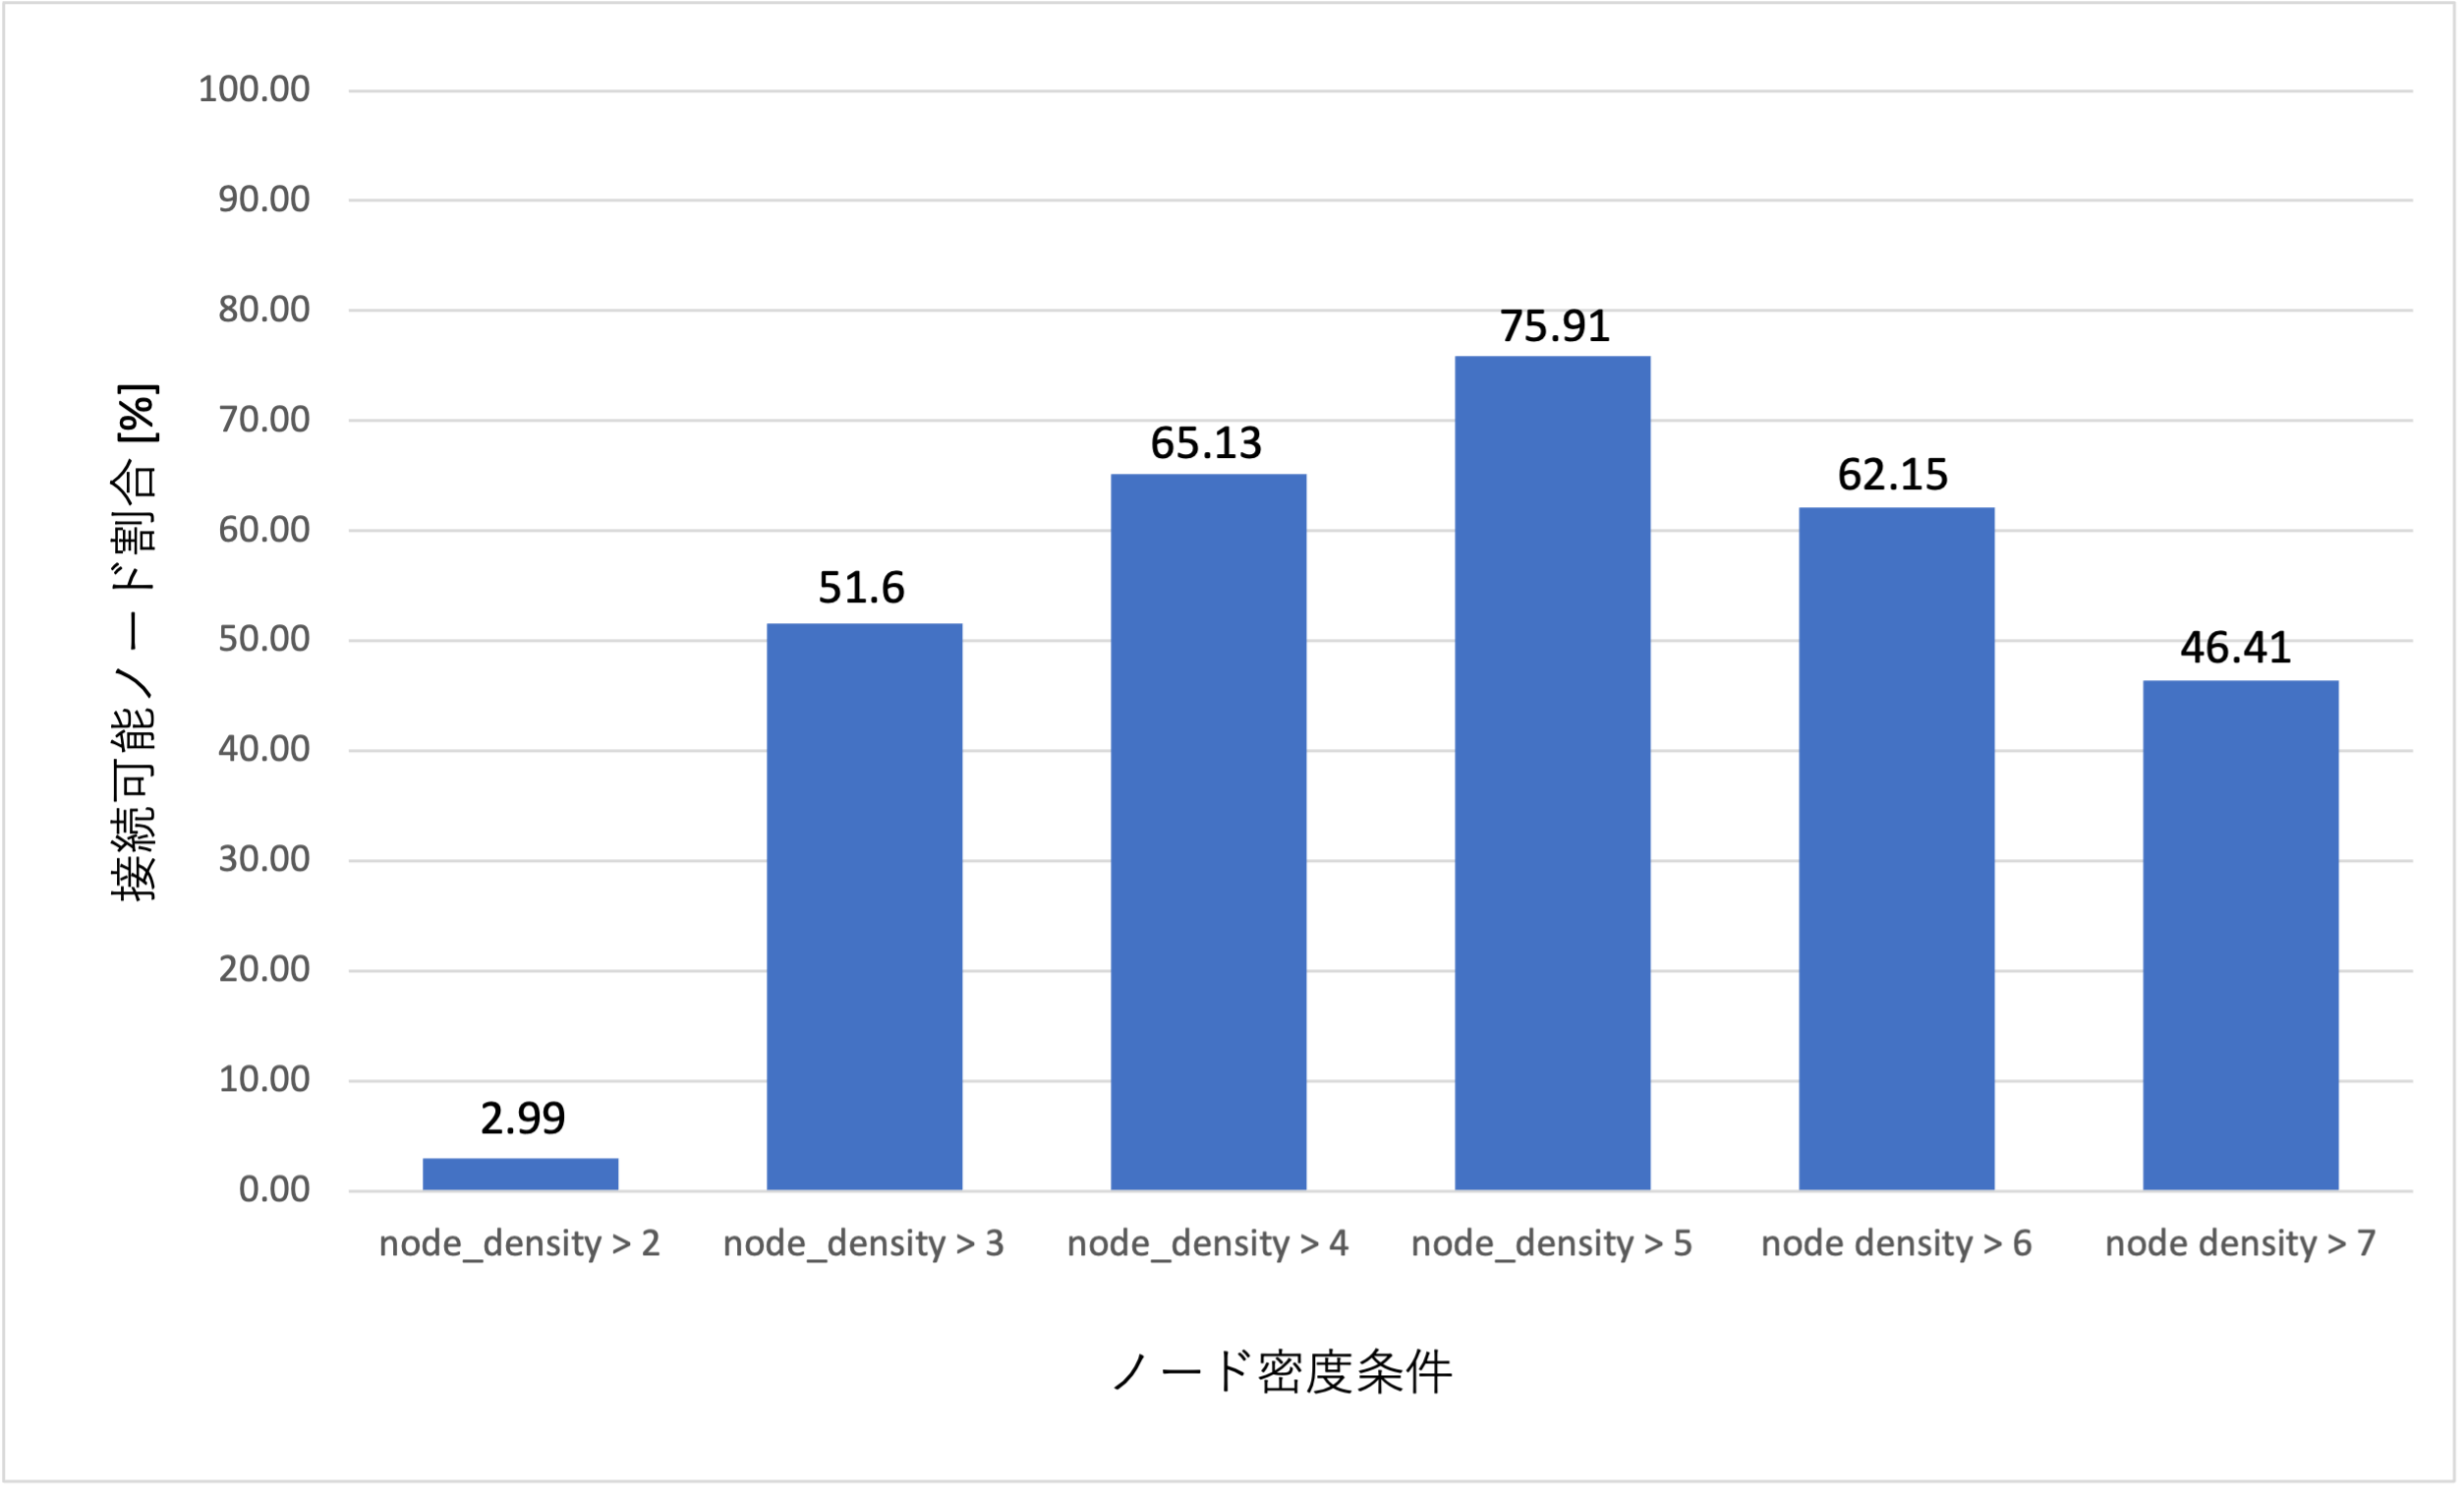
\includegraphics[width=80mm]{提案1の結果.png}
  \caption{提案手法-1のシミュレーション結果}
  \label{fig:1} % 参照用のラベル
\end{figure}

\begin{figure}[ht]
  \centering
  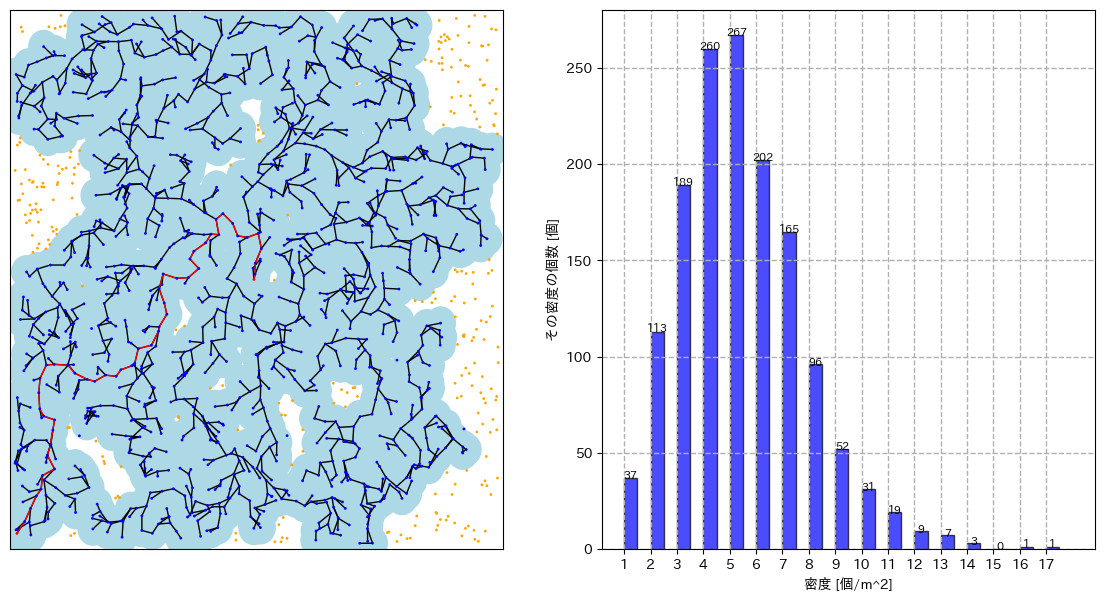
\includegraphics[width=80mm]{simulation_result.png}
  \caption{$\mathrm{node\_density>5}$のシミュレーションの様子}
  \label{fig:2}
\end{figure}

\subsection{提案手法-2}
次に、提案手法-1に電柱ノードを追加した際のシミュレーションを行った。電柱ノードには特に追加の条件は与えなかった。
この提案手法では、ノード数の増加による成功率の上昇具合について知るのが目的である。


\section{考察}
提案手法-1のシミュレーション結果より、周辺ノードの密度が4\textasciitilde6のとき経路生成が多く行われることがわかった。
しかし、図\ref{fig:2}のようにノードの位置が均一になっていないため密から疎の地域へ通信を拡大することができなかった。
そのため、今後の課題として電柱や街灯等の動かずかつ、一定間隔に設置されているシンボルにノードを設置することでノードの総数を
増やす必要があると考えられる。

\section{まとめ}
本研究では、災害時を想定したアドホックネットワーク構築する際、多量のノードにより複雑化してしまう経路を
下流ノードの接続状況と周辺のノード密度を考慮することにより簡単な経路探索する手法を検討した。
その結果、周辺ノードの密度が4\textasciitilde6であるとき広範囲なネットワークを生成することができた。
また、ループが発生しないため通信品質も保つことができると考えられる。しかし、スタートノード周辺のノードの負荷が大きくなってしまうため、
複数のスタートノードを用意し、負荷の分散を行う必要があると考えられる。\par
今回のシミュレーションでは、アドホックネットワークの技術的課題について触れていないため実際の環境では異なる結果が出ると考えられるため、
今後は実環境で実験を行いそれを元にシミュレーションを改良していきたいと考えている。

\begin{thebibliography}{9}
  \bibitem{スマホ保有率} \url{https://www.soumu.go.jp/johotsusintokei/whitepaper/ja/r04/html/nd238110.html}, 総務省, 「通信利用動向調査」 
  \bibitem{電柱設置間隔} \url{https://www.tepco.co.jp/pg/company/press-information/press/2019/pdf/190808j0101.pdf}, 東京電力, 「全国の「位置情報データ」の代理店販売の概要」
  \bibitem{人口密度} \url{https://uub.jp/rnk/p\_j.html}, 都道府県市区町村, 「都道府県 人口・面積・人口密度ランキング」
\end{thebibliography}

\end{document}
